% Explainer for stochastic declustering. Build from this folder: tectonic algorithm_explainer.tex
% Figure data and worked-example numbers come from scripts/explainer_data.py.
\documentclass[11pt,a4paper]{article}
\usepackage[margin=2.3cm]{geometry}
\usepackage{amsmath,amssymb,booktabs,array,xcolor,microtype,parskip,float}
\usepackage{tikz,pgfplots}
\usepackage[hidelinks]{hyperref}
\usetikzlibrary{arrows.meta,positioning,shapes.geometric,fit,backgrounds,calc}
\pgfplotsset{compat=1.18}
\pgfdeclarelayer{back}\pgfsetlayers{back,background,main}

\definecolor{ink}{HTML}{0B0B0B}
\definecolor{muted}{HTML}{52514E}
\definecolor{gridline}{HTML}{E4E3DF}
\definecolor{bg}{HTML}{2A78D6}   % background events
\definecolor{trig}{HTML}{EB6834} % triggered events, and the costly step
\definecolor{boxfill}{HTML}{F5F5F2}

\newcommand{\code}[1]{\texttt{#1}}
\newcommand{\mo}{m}
\newcommand{\dd}{\,\mathrm{d}}

\title{Stochastic declustering, from the problem to the algorithm}
\author{Companion to \code{etas8py}, a port of Zhuang's Fortran code}
\date{5 November 2026}

\begin{document}
\maketitle

\section{The problem}

Earthquakes do not arrive independently. A large earthquake is followed by aftershocks, those
aftershocks have aftershocks of their own, and a catalogue ends up as a mix of two populations:

\begin{itemize}
  \item \textbf{Background events}, driven by slow tectonic loading. Their rate is roughly constant
  in time but varies a lot from place to place.
  \item \textbf{Triggered events}, set off by an earlier earthquake. They bunch tightly in
  time and space around their parent.
\end{itemize}

\textbf{Declustering} means separating the two. It matters because the clusters hide the
long-term signal: to map where stress steadily accumulates, or to ask whether the seismicity rate
really changed, you need to look at the background without the aftershock bursts on top of it.

The catalogue does not tell you which event is which. Each row is only a time, a place and a
magnitude. Most older methods draw a space-time window around each large event and delete
everything inside it; others link events that are close in space and time. Both force a yes/no
answer for every event and depend on hand-picked window sizes or link distances.

\textbf{Stochastic declustering} replaces the yes/no with a probability. A statistical model
of how earthquakes trigger each other is fitted to the catalogue, and it then gives each event a
probability $\varphi_i$ of being background.

\begin{figure}[H]
\centering
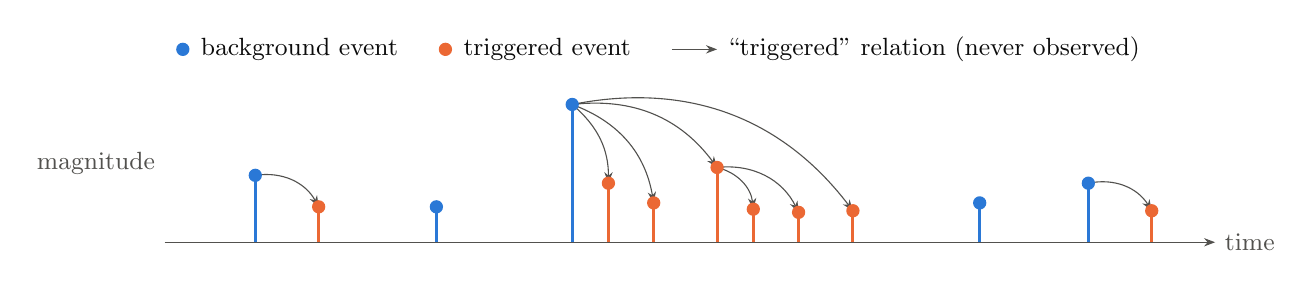
\begin{tikzpicture}[x=1.15cm,y=1cm,>={Stealth[length=4pt]}]
  \draw[muted,->] (0,0) -- (11.6,0) node[right,font=\small] {time};
  \newcommand{\ev}[3]{\draw[#3,line width=1.1pt] (#1,0) -- (#1,#2); \fill[#3] (#1,#2) circle (2.4pt);}
  \newcommand{\link}[5]{\draw[->,muted,thin] (#1,#2) to[bend left=#5] (#3,#4);}
  \link{1}{.85}{1.7}{.45}{35}
  \link{4.5}{1.75}{4.9}{.75}{25}
  \link{4.5}{1.75}{5.4}{.5}{30}
  \link{4.5}{1.75}{6.1}{.95}{30}
  \link{4.5}{1.75}{7.6}{.4}{32}
  \link{6.1}{.95}{6.5}{.42}{35}
  \link{6.1}{.95}{7.0}{.38}{35}
  \link{10.2}{.75}{10.9}{.4}{35}
  \ev{1}{.85}{bg}\ev{4.5}{1.75}{bg}\ev{9}{.5}{bg}\ev{10.2}{.75}{bg}\ev{3}{.45}{bg}
  \ev{1.7}{.45}{trig}\ev{4.9}{.75}{trig}\ev{5.4}{.5}{trig}\ev{6.1}{.95}{trig}\ev{7.6}{.4}{trig}
  \ev{6.5}{.42}{trig}\ev{7.0}{.38}{trig}\ev{10.9}{.4}{trig}
  \fill[bg] (.2,2.45) circle (2.4pt) node[right=3pt,ink,font=\small] {background event};
  \fill[trig] (3.1,2.45) circle (2.4pt) node[right=3pt,ink,font=\small] {triggered event};
  \draw[->,muted,thin] (5.6,2.45) -- (6.1,2.45) node[right,ink,font=\small] {``triggered'' relation (never observed)};
  \node[left,font=\small,muted] at (0,1) {magnitude};
\end{tikzpicture}
\caption{The hidden structure. Real data shows only the stems, with no colours and no arrows.
Note the chains: an aftershock can have aftershocks.}
\end{figure}

\paragraph{The chicken-and-egg difficulty.}
To label the events you need the background rate and the triggering rules. To estimate those you
need the labels. The algorithm breaks the loop by guessing one side, computing the other, and
repeating until nothing changes. Sections 2--4 define the pieces and Section 5 shows the loop.

\section{Language: rates and likelihood}

A \textbf{conditional intensity} $\lambda(t,x,y)$ is the expected number of events per day per square
degree at that time and place, given everything that happened before. Integrating $\lambda$ over a
region and time window gives the expected number of events there.

The fit quality of a candidate model on the target events is its \textbf{log-likelihood}:
\begin{equation}
  \log L \;=\; \sum_{i\,\in\,\text{targets}} \log \lambda(t_i,x_i,y_i)
  \;-\; \int_{\text{window}}\!\!\iint_{S} \lambda(t,x,y) \dd x\dd y\dd t .
  \label{eq:logL}
\end{equation}
The first term rewards a high rate where earthquakes did happen. The second term penalises the
total number of events the model predicted, so the rate cannot simply be raised everywhere. The
second term is what makes this code expensive (Section~6).

\section{The model: ETAS}

\textbf{Epidemic-Type Aftershock Sequence} treats earthquakes like an epidemic: every event, large
or small, can ``infect'' the future. With $m_j = M_j - M_0$ the magnitude above the catalogue
cutoff, the intensity is a background term plus one term per earlier event:
\begin{equation}
  \lambda(t,x,y) = \underbrace{\mu\,u(x,y)}_{\text{background}}
  + \sum_{t_j<t} \kappa_j(t,x,y),
  \label{eq:lambda}
\end{equation}
\begin{equation}
  \kappa_j(t,x,y) =
  \underbrace{A e^{\alpha m_j}}_{\substack{\text{how many}\\\text{children}}}
  \cdot
  \underbrace{\frac{p-1}{c}\Bigl(1+\frac{t-t_j}{c}\Bigr)^{-p}}_{\substack{\text{when: Omori--Utsu decay}}}
  \cdot
  \underbrace{\frac{q-1}{\pi D e^{\gamma m_j}}\Bigl(1+\frac{r_j^2}{D e^{\gamma m_j}}\Bigr)^{-q}}_{\substack{\text{where: spreads with magnitude}}}
  \label{eq:kappa}
\end{equation}
where $r_j$ is the distance to event $j$. The ``when'' and ``where'' factors each integrate to 1,
so $A e^{\alpha m_j}$ is the expected total number of children of event $j$, over all time and space.

\begin{table}[H]
\centering\small
\begin{tabular}{@{}lll@{}}
\toprule
Parameter & Meaning & Fitted value (JMA example) \\
\midrule
$\mu$ & scales the background term & 0.551 \\
$A$ & children of an event at the cutoff magnitude & 0.166 \\
$\alpha$ & how fast productivity grows with magnitude & 1.658 \\
$c$ & short delay before the decay starts & 0.0296 days (43 min) \\
$p$ & how fast the rate decays in time & 1.153 \\
$D$ & spatial scale at the cutoff magnitude & 0.00183 deg$^2$ = 22.7 km$^2$ \\
$q$ & how fast the rate decays with distance & 1.951 \\
$\gamma$ & how fast the spatial scale grows with magnitude & 1.067 \\
\bottomrule
\end{tabular}
\caption{The eight ETAS parameters, $\theta = (\mu,A,c,\alpha,p,D,q,\gamma)$, from \code{results/cfg\_default\_flat}.}
\end{table}

Those values mean that magnitude dominates everything, as this table of $A e^{\alpha m}$ and
$\sqrt{D e^{\gamma m}}$ shows:

\begin{table}[H]
\centering\small
\begin{tabular}{@{}lrrrrr@{}}
\toprule
Magnitude & 4.5 & 5.5 & 6.5 & 7.5 & 8.2 \\
\midrule
Expected direct children & 0.17 & 0.87 & 4.57 & 24.0 & 76.5 \\
Spatial scale (km) & 4.8 & 8.1 & 13.8 & 23.6 & 34.3 \\
\bottomrule
\end{tabular}
\caption{Productivity and spatial scale implied by the fitted parameters.}
\end{table}

\paragraph{The background $u(x,y)$.}
No formula is assumed for the background map. It is built from the data by placing a small
Gaussian bump on every event and weighting it by the probability that the event is background:
\begin{equation}
  u(x,y) = \frac{1}{T_{\text{window}}}\sum_j \varphi_j \, g_{h_j}\!\bigl(r_j\bigr),
  \qquad g_h(r) = \frac{1}{2\pi h^2}\,e^{-r^2/2h^2}.
  \label{eq:u}
\end{equation}
$T_{\text{window}}$ is the length of the target window (13376 days for JMA). This is a \textbf{variable-bandwidth kernel density estimate}. The width $h_j$ is the distance from
event $j$ to its 5th nearest neighbour, floored at $0.05^\circ$ (5.6 km). Crowded areas get sharp
bumps and empty areas get wide ones. On JMA the median is 7.4 km and the 99th percentile 60 km,
and 3542 of the 10071 events sit on the floor. The sum includes the event itself, as in the original.

Equation~\eqref{eq:u} is where the circularity sits: $u$ needs $\varphi$, and
$\varphi$ (next section) needs $u$.

\section{From the model to probabilities}

Equation~\eqref{eq:lambda} says the rate at event $i$ is a sum of separate causes. If causes add
up as rates, the probability that a given cause produced the event is its share of the total:
\begin{equation}
  \underbrace{\varphi_i = \frac{\mu\,u(x_i,y_i)}{\lambda(t_i,x_i,y_i)}}_{\text{event $i$ is background}}
  \qquad\qquad
  \underbrace{\rho_{ij} = \frac{\kappa_j(t_i,x_i,y_i)}{\lambda(t_i,x_i,y_i)}}_{\text{event $i$ was triggered by $j$}}
  \qquad\qquad
  \varphi_i + \sum_{j<i}\rho_{ij} = 1.
  \label{eq:phi}
\end{equation}

\paragraph{Three real events from the JMA run.} Rates are per day per deg$^2$.

\begin{table}[H]
\centering\small
\begin{tabular}{@{}lrrrl@{}}
\toprule
Event & $\mu u_i$ & $\lambda_i$ & $\varphi_i$ & Largest triggering share $\rho_{ij}$ \\
\midrule
\#4461, M5.1 & 0.00185 & 0.1067 & 0.017 & 0.72: a M7.4, 2 days earlier, 64 km away \\
\#7048, M4.6 & 0.00075 & 0.00159 & 0.470 & 0.51: a M5.0, 0.32 days earlier, 71 km away \\
\#5950, M5.0 & 0.03091 & 0.03218 & 0.960 & 0.007: a M4.7, 2014 days earlier, 3.5 km away \\
\bottomrule
\end{tabular}
\caption{Each row asks what share of the rate at that event comes from the background. The second
event is genuinely ambiguous, which a window method cannot express.}
\label{tab:events}
\end{table}

\paragraph{Why ``stochastic''.}
To get an actual declustered catalogue, draw a uniform random number $U_i$ for each event and keep
it as background if $U_i<\varphi_i$. Otherwise it is triggered, and you can pick its parent $j$ with
probability $\rho_{ij}/(1-\varphi_i)$. These are Algorithms 2 and 3 of the paper. Each draw gives
one equally plausible catalogue, and repeating the draw shows how uncertain any conclusion is. The
paper stresses that the essential output is the probabilities, not any one catalogue. This code
computes $\varphi_i$ and stops there: the random draw is not implemented, and the Python port does
not write the $\rho_{ij}$ matrix (the original's \code{pmatr.dat}).

\section{The algorithm}

The loop has two levels. The inner one solves the circularity between $u$ and $\varphi$ with the
parameters frozen. The outer one re-fits the parameters with $u$ frozen, then goes round again.
In spirit this is like expectation--maximisation (assign events to causes, re-fit, repeat), but it
is not formally EM. Figure~\ref{fig:flow} shows the whole thing.

\begin{figure}[p]
\centering
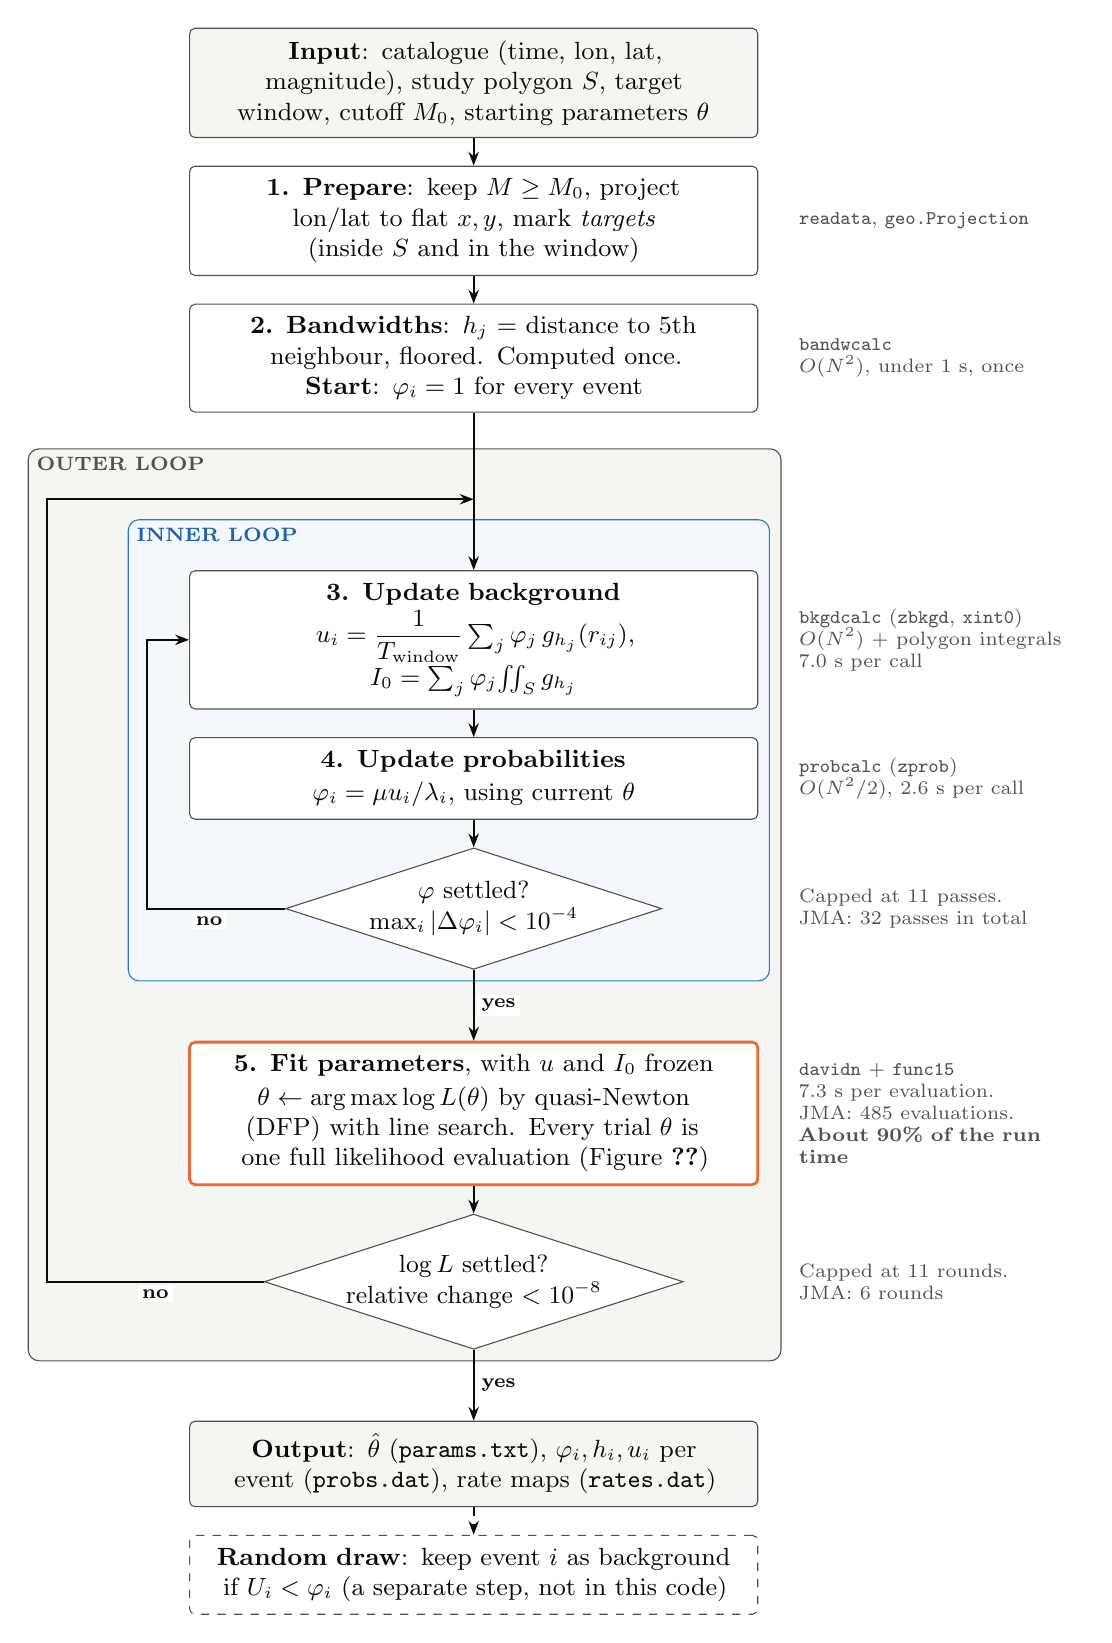
\begin{tikzpicture}[
  >={Stealth[length=5pt]},
  box/.style={draw=muted,fill=white,rounded corners=2pt,align=center,text width=6.9cm,
              inner sep=4.5pt,font=\small,execute at begin node={\thickmuskip=5mu\hyphenpenalty=10000\relax}},
  io/.style={box,fill=boxfill},
  dec/.style={draw=muted,fill=white,diamond,aspect=3.1,align=center,inner sep=0pt,font=\small},
  hot/.style={box,draw=trig,line width=1pt},
  note/.style={align=left,text width=3.5cm,font=\scriptsize,text=muted,anchor=west,
               execute at begin node={\hyphenpenalty=10000\relax}},
  flow/.style={->,line width=.7pt,draw=ink},
  lbl/.style={font=\scriptsize\bfseries,fill=white,inner sep=1.5pt},
  every node/.append style={text=ink}]

  \node[io] (in) {\textbf{Input}: catalogue (time, lon, lat, magnitude), study polygon $S$,
    target window, cutoff $M_0$, starting parameters $\theta$};
  \node[box,below=3.5mm of in] (prep) {\textbf{1. Prepare}: keep $M\ge M_0$, project lon/lat to flat
    $x,y$, mark \emph{targets} (inside $S$ and in the window)};
  \node[box,below=3.5mm of prep] (bw) {\textbf{2. Bandwidths}: $h_j$ = distance to 5th neighbour,
    floored. Computed once.\\ \textbf{Start}: $\varphi_i=1$ for every event};
  \coordinate[below=11mm of bw] (J);
  \node[box,below=9mm of J] (C) {\textbf{3. Update background}\\[1pt]
    $u_i = \dfrac{1}{T_{\text{window}}}\sum_j \varphi_j\, g_{h_j}(r_{ij})$,\quad
    $I_0=\sum_j \varphi_j\!\iint_S g_{h_j}$};
  \node[box,below=3.5mm of C] (D) {\textbf{4. Update probabilities}\\[1pt]
    $\varphi_i = \mu u_i/\lambda_i$, using current $\theta$};
  \node[dec,below=3.5mm of D] (d1) {$\varphi$ settled?\\ $\max_i|\Delta\varphi_i|<10^{-4}$};
  \node[hot,below=9mm of d1] (E) {\textbf{5. Fit parameters}, with $u$ and $I_0$ frozen\\[1pt]
    $\theta \leftarrow \arg\max \log L(\theta)$ by quasi-Newton (DFP) with line search.
    Every trial $\theta$ is one full likelihood evaluation (Figure~\ref{fig:zoom})};
  \node[dec,below=3.5mm of E] (d2) {$\log L$ settled?\\ relative change $<10^{-8}$};
  \node[io,below=9mm of d2] (out) {\textbf{Output}: $\hat\theta$ (\code{params.txt}), $\varphi_i, h_i, u_i$
    per event (\code{probs.dat}), rate maps (\code{rates.dat})};
  \node[box,below=3.5mm of out,dashed] (thin) {\textbf{Random draw}: keep event $i$ as background if
    $U_i<\varphi_i$ (a separate step, not in this code)};

  % Arrows on the main path
  \draw[flow] (in) -- (prep); \draw[flow] (prep) -- (bw);
  \draw[flow] (bw) -- (C);
  \draw[flow] (C) -- (D); \draw[flow] (D) -- (d1);
  \draw[flow] (d1) -- node[lbl,right=1pt] {yes} (E);
  \draw[flow] (E) -- (d2);
  \draw[flow] (d2) -- node[lbl,right=1pt] {yes} (out);
  \draw[flow,dashed] (out) -- (thin);

  % Loop-backs
  \draw[flow] (d1.west) -- node[lbl,pos=.55,below=1pt] {no} ++(-1.75,0) coordinate (a) |- (C.west);
  \draw[flow] (d2.west) -- node[lbl,pos=.5,below=1pt] {no} ++(-2.75,0) coordinate (b) |- (J);

  % Loop containers, drawn behind
  \coordinate (al) at ($(a)+(-.1,0)$); \coordinate (bl) at ($(b)+(-.1,0)$);
  \coordinate (ct) at ($(C.north)+(0,5mm)$); \coordinate (jt) at ($(J)+(0,5mm)$);
  \begin{scope}[on background layer]
    \node[draw=bg,fill=bg!5,rounded corners=4pt,inner xsep=4pt,inner ysep=4pt,
          fit=(C)(D)(d1)(al)(ct),
          label={[anchor=north west,font=\scriptsize\bfseries,text=bg!80!black,inner sep=3pt]north west:INNER LOOP}] (inner) {};
    \begin{pgfonlayer}{back}
      \node[draw=muted,fill=boxfill,rounded corners=4pt,inner xsep=4pt,inner ysep=4pt,
          fit=(inner)(E)(d2)(bl)(jt),
          label={[anchor=north west,font=\scriptsize\bfseries,text=muted,inner sep=3pt]north west:OUTER LOOP}] (outer) {};
    \end{pgfonlayer}
  \end{scope}

  % Margin notes: code names and costs
  \node[note] at ($(outer.east |- prep)+(1mm,0)$) {\code{readata}, \code{geo.Projection}};
  \node[note] at ($(outer.east |- bw)+(1mm,0)$) {\code{bandwcalc}\\ $O(N^2)$, under 1 s, once};
  \node[note] at ($(outer.east |- C)+(1mm,0)$) {\code{bkgdcalc} (\code{zbkgd}, \code{xint0})\\ $O(N^2)$ + polygon integrals\\ 7.0 s per call};
  \node[note] at ($(outer.east |- D)+(1mm,0)$) {\code{probcalc} (\code{zprob})\\ $O(N^2/2)$, 2.6 s per call};
  \node[note] at ($(outer.east |- d1)+(1mm,0)$) {Capped at 11 passes.\\ JMA: 32 passes in total};
  \node[note] at ($(outer.east |- E)+(1mm,0)$) {\code{davidn} + \code{func15}\\ 7.3 s per evaluation.\\ JMA: 485 evaluations.\\ \textbf{About 90\% of the run time}};
  \node[note] at ($(outer.east |- d2)+(1mm,0)$) {Capped at 11 rounds.\\ JMA: 6 rounds};
\end{tikzpicture}
\caption{The whole algorithm. Timings are single-thread per-call measurements on the JMA catalogue
($N=10071$), from the clean rerun in \code{architecture.md}. The original Fortran has no
convergence tests: it runs a fixed schedule of 11 outer rounds with 11, 10, \dots, 1 inner passes.}
\label{fig:flow}
\end{figure}

\subsection*{Walking through the boxes}

\textbf{Step 1, prepare.} Targets are the events whose fit we score: inside the polygon and inside
the target window (1953--1990 for JMA). The other events are not thrown away. Earlier events and
those outside the polygon can still trigger targets, so they stay in the sums in
Equation~\eqref{eq:lambda}. JMA keeps 10071 events, of which 4656 are targets. The projection is
where \code{flat} (the original) or \code{laea} (equal-area) is applied.

\textbf{Step 2, bandwidths.} These depend only on event locations, so they never change.

\textbf{Step 3, background.} Applies Equation~\eqref{eq:u} at every event. On the first pass all
$\varphi_j=1$, so $u$ is a map of all seismicity, clusters included. It also computes
$I_0$, the background's weight inside the polygon, which Step 5 reuses.

\textbf{Step 4, probabilities.} Applies Equation~\eqref{eq:phi}. Events near big shocks get low
$\varphi_i$. Back in Step 3 they then contribute less to $u$, so the map loses its
aftershock peaks, and the next $\varphi_i$ change a little less. On JMA the largest change
falls from 1.0 on pass 1 to $4.7\times10^{-4}$ on pass 11.

\textbf{Step 5, fit.} With $u$ frozen, Equation~\eqref{eq:logL} is an ordinary function of eight
numbers, and an optimiser climbs it. The optimiser works on $\sqrt\theta$, which keeps every
parameter positive without constraints. New parameters change $\lambda$, hence $\varphi$, hence
$u$, so the outer loop goes back to Step 3.

\textbf{Stopping.} The paper stops when the largest change in $u$ falls below a small number. The
Fortran has no test and runs a fixed schedule. The tests shown here are this project's choice, and
can be turned off to reproduce the Fortran. Both agree closely on JMA: parameters within $1.4\times10^{-6}$ (relative)
and $\varphi$ within $8.4\times10^{-6}$. The $\varphi_i$ in \code{probs.dat} come from the last
pass, just before the final fit, as in the original. At convergence that gap is negligible:
recomputing the three events in Table~\ref{tab:events} with the final $\theta$ gives the same values.

\section{Why it is slow: the polygon integrals}

The penalty term in Equation~\eqref{eq:logL} has to be recomputed for each trial $\theta$:
\begin{equation}
  \underbrace{\mu I_0}_{\text{stored from Step 3}}
  + \sum_{j} A e^{\alpha m_j}
  \underbrace{G_j}_{\substack{\text{time integral,}\\\text{closed form}}}
  \quad\underbrace{S_j}_{\substack{\text{space integral of \eqref{eq:kappa}'s}\\\text{``where'' factor over $S$}}}
\end{equation}

$S_j$ asks: what fraction of event $j$'s aftershocks land inside the study polygon? There is no
closed form for that, because the kernel is circular and the polygon is not.


\begin{minipage}[t]{.47\linewidth}
\vspace{0pt}\centering
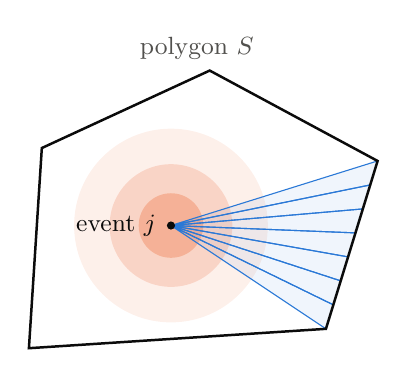
\begin{tikzpicture}[scale=.82]
  \coordinate (E) at (2.2,1.9);
  \coordinate (P1) at (0,0); \coordinate (P2) at (4.6,.3); \coordinate (P3) at (5.4,2.9);
  \coordinate (P4) at (2.8,4.3); \coordinate (P5) at (.2,3.1);
  \foreach \r/\o in {.5/32,.95/20,1.5/10} \fill[trig,opacity=.\o] (E) circle (\r);
  \foreach \k in {0,...,6} {
    \coordinate (A) at ($(P2)!{\k/7}!(P3)$);
    \coordinate (B) at ($(P2)!{(\k+1)/7}!(P3)$);
    \draw[bg,fill=bg,fill opacity=.07,thin] (E) -- (A) -- (B) -- cycle;
  }
  \draw[ink,line width=.9pt] (P1)--(P2)--(P3)--(P4)--(P5)--cycle;
  \fill[ink] (E) circle (1.8pt) node[left=2pt,font=\small] {event $j$};
  \node[font=\small,muted] at (2.6,4.65) {polygon $S$};
\end{tikzpicture}
\end{minipage}\hfill
\begin{minipage}[t]{.5\linewidth}
\vspace{4pt}
\textbf{The trick.} By Green's theorem the area integral becomes a sum over the boundary. Each
edge is cut into 1000 pieces, and each piece forms a thin triangle with the event. A radial
kernel has a closed-form antiderivative $F(r)$, so each triangle needs only a one-dimensional
Simpson rule in the angle. Triangle areas are signed, so an event outside the polygon also works:
parts of the fan cancel. The figure shows the fan for one edge, with 7 pieces rather than 1000.

\smallskip
\textbf{The cost.} 27000 radial evaluations per integral in the original, four integrals per
event, 10071 events: about $1.1\times10^9$ per evaluation, hundreds of times over.
\end{minipage}

\medskip
This is why the project's first speedup targeted this step, sharing work between the four
integrals and between neighbouring pieces. Full-run time at 10 cores went from 3965 s (Fortran MPI)
to 940 s (Python), with results matching to about $10^{-6}$. The $O(N^2)$ pair sums are next. Figure~\ref{fig:zoom} shows where this step sits in one likelihood evaluation.

\begin{figure}[H]
\centering
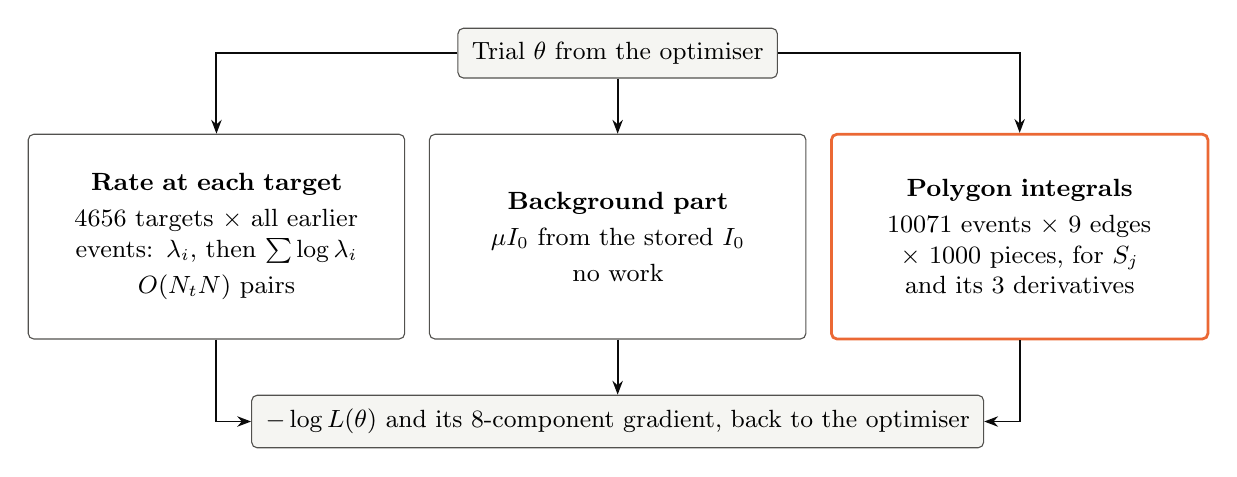
\begin{tikzpicture}[
  >={Stealth[length=5pt]},
  box/.style={draw=muted,fill=white,rounded corners=2pt,align=center,text width=4.5cm,
              inner sep=4pt,font=\small,minimum height=2.6cm},
  flow/.style={->,line width=.7pt,draw=ink}]
  \node[draw=muted,fill=boxfill,rounded corners=2pt,inner sep=5pt,font=\small] (th) {Trial $\theta$ from the optimiser};
  \node[box,below=7mm of th] (b) {\textbf{Background part}\\[2pt]$\mu I_0$ from the stored $I_0$\\[2pt]
     no work};
  \node[box,left=3mm of b] (a) {\textbf{Rate at each target}\\[2pt]
     4656 targets $\times$ all earlier events: $\lambda_i$, then $\sum \log\lambda_i$\\[2pt]
     $O(N_t N)$ pairs};
  \node[box,right=3mm of b,draw=trig,line width=1pt] (c) {\textbf{Polygon integrals}\\[2pt]
     10071 events $\times$ 9 edges $\times$ 1000 pieces, for $S_j$ and its 3 derivatives};
  \node[draw=muted,fill=boxfill,rounded corners=2pt,inner sep=5pt,font=\small,below=7mm of b] (f)
     {$-\log L(\theta)$ and its 8-component gradient, back to the optimiser};
  \draw[flow] (th) -| (a); \draw[flow] (th) -- (b); \draw[flow] (th) -| (c);
  \draw[flow] (a) |- (f); \draw[flow] (b) -- (f); \draw[flow] (c) |- (f);
\end{tikzpicture}
\caption{One likelihood evaluation (\code{func15}). Polygon integrals took 31.0 of 33.5 s in
the 1:1 port and 6.6 of 8.7 s after this project's fused version.}
\label{fig:zoom}
\end{figure}

\section{What comes out on JMA}

\begin{figure}[H]
\centering
\begin{tikzpicture}
\begin{axis}[width=.88\linewidth,height=6.2cm,clip=false,
  xlabel={Year},ylabel={Cumulative target events},
  xmin=1953,xmax=1990.2,ymin=0,ymax=5000,
  xtick={1955,1960,...,1990},
  /pgf/number format/1000 sep={},
  scaled y ticks=false,
  axis lines=left,axis line style={muted},tick style={muted},
  tick label style={font=\small,text=muted},label style={font=\small},
  ymajorgrids,grid style={gridline},
  legend style={at={(.02,.98)},anchor=north west,draw=none,font=\small,fill=white},
  legend cell align=left]
  \addplot[trig,line width=1.1pt,no markers] table[x=year,y=all] {explainer_cum.dat};
  \addlegendentry{All target events}
  \addplot[bg,line width=1.1pt,no markers] table[x=year,y=background] {explainer_cum.dat};
  \addlegendentry{Expected background ($\sum\varphi_i$)}
  \node[anchor=west,font=\small] at (axis cs:1990.4,4656) {4656};
  \node[anchor=west,font=\small] at (axis cs:1990.4,2347.5) {2347.5};
\end{axis}
\end{tikzpicture}
\caption{Declustering removes the jumps. The largest step is the M7.9 of 1968: 277 target events in
60 days, but only 19.7 expected background events. The M7.7 of 1983 gives 183 events and 11.3.
Source: \code{results/cfg\_default\_flat/probs.dat}, \code{scripts/explainer\_data.py}.}
\label{fig:cum}
\end{figure}

\begin{minipage}[t]{.5\linewidth}
\vspace{0pt}\centering
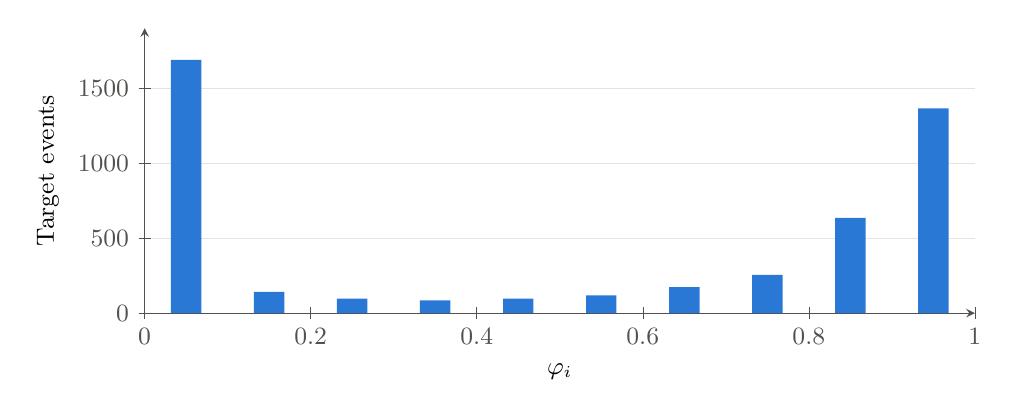
\begin{tikzpicture}
\begin{axis}[width=\linewidth,height=5.2cm,ybar,bar width=11pt,
  xlabel={$\varphi_i$},ylabel={Target events},
  xmin=0,xmax=1,ymin=0,ymax=1900,xtick={0,.2,.4,.6,.8,1},
  /pgf/number format/1000 sep={},
  enlarge x limits=.04,
  axis lines=left,axis line style={muted},tick style={muted},
  tick label style={font=\small,text=muted},label style={font=\small},
  ymajorgrids,grid style={gridline}]
  \addplot[fill=bg,draw=none] coordinates {(.05,1689)(.15,141)(.25,97)(.35,85)(.45,96)(.55,118)(.65,174)(.75,255)(.85,636)(.95,1365)};
\end{axis}
\end{tikzpicture}
\end{minipage}\hfill
\begin{minipage}[t]{.46\linewidth}
\vspace{6pt}
\textbf{Most events are clear-cut.} Of 4656 targets, 1689 have $\varphi_i<0.1$ and 1365 have
$\varphi_i>0.9$. The other 1602 are ambiguous, and a yes/no window method would hide that.

\smallskip
\textbf{About half is background.} Expected background is $\sum\varphi_i=2347.5$ of 4656, or 50.4\%.

\smallskip
\textbf{A built-in check.} Setting $\partial\log L/\partial\mu=0$ gives
$\sum_{\text{targets}}\varphi_i=\mu I_0$ at the optimum. Here the two sides are 2347.5239 and
2347.5237.
\end{minipage}

\medskip
\paragraph{Why $\mu\approx0.55$, not 1.}
Equation~\eqref{eq:u} sums over all events since 1926 but divides by the target window only (13376
days). Taken at face value that overstates the daily background rate by about $23376/13376$, so
$\mu$ should come out near $13376/23376=0.57$, and it does. The paper supports this: where its sum
and its $T$ cover the same period (New Zealand), the same factor converges to 0.9997. It is still
my inference, as the paper does not discuss this case. The choice is harmless, because only the
product $\mu u$ enters the likelihood and $\varphi_i$, so $\mu$ absorbs any constant rescaling of $u$.

\section{How this code differs from the paper}
\label{sec:paper}

The model and algorithm in this document follow the code. They are checked here against Zhuang,
Ogata \& Vere-Jones (2002) and its follow-up (2004). The probabilities $\varphi_i,\rho_{ij}$, the
weighted kernel estimate and the idea of alternating between $u$ and $\theta$ all match the 2002 paper.
These details do not:

\begin{table}[H]
\centering\small
\begin{tabular}{@{}l>{\raggedright\arraybackslash}p{5.3cm}>{\raggedright\arraybackslash}p{5.9cm}@{}}
\toprule
 & 2002 paper & This code \\
\midrule
Spatial kernel & Gaussian, sharing $\alpha$ with productivity (6 parameters) &
  Power law with $q$ and its own $\gamma$ (8 parameters). The 2004 paper has the power law, but still with shared $\alpha$ \\
Loop & One loop: fit $\theta$, then $\rho$, then $u$ & Two levels: $u$ and $\varphi$ until settled, then fit $\theta$ \\
Start & $u=1$, so the first step is a fit & $\varphi=1$, so the first step is $u$ \\
Stopping & $\max|\Delta u|<\varepsilon$ & Fortran: fixed schedule. This port: $\Delta\varphi$ and $\Delta\log L$ tests \\
Bandwidth & $n_p=20$, floor $0.02^\circ$ & $n_p=5$, floor $0.05^\circ$, the values suggested in the 2004 paper \\
$T$ in $u$ & Length of the observation period & Target window only, with the sum over all events \\
Output & Declustered catalogues and family trees (Algorithms 2, 3) & $\varphi_i$ only \\
\bottomrule
\end{tabular}
\caption{Differences found by reading both papers. I did not trace which later paper introduced
the separate $\gamma$. The Fortran itself is the source for the code's form.}
\end{table}

\section{Symbols and where they live in the code}
\begin{table}[H]
\centering\small
\begin{tabular}{@{}lll@{}}
\toprule
Symbol & Meaning & Code name \\
\midrule
$\mu$ & scale of the background term; the paper's $\nu$ & \code{b(1)}, \code{mu} \\
$\rho_{ij}$ & event $i$ triggered by $j$; the paper writes $\rho_{j,i}$ & not computed \\
$\varphi_i$ & probability event $i$ is background & \code{zprob}, \code{background\_prob} \\
$u_i$ & background density at event $i$, per day & \code{zbkgd}, \code{background\_rate} \\
$h_j$ & Gaussian bandwidth of event $j$ & \code{zbandw}, \code{bandwidth} \\
$I_0$ & $\sum_j\varphi_j\iint_S g_{h_j}$ & \code{xint0} \\
$\lambda_i$ & total intensity at event $i$ & \code{xlamb} \\
$G_jS_j$ & time and space integrals of event $j$'s offspring & \code{xint}, \code{xint\_fast} \\
$S_j$ & one polygon integral & \code{polyint}, \code{frint} \\
$-\log L$ & objective and gradient & \code{func15} \\
targets & events scored in $\sum\log\lambda_i$ & \code{ind == 1} \\
\bottomrule
\end{tabular}
\end{table}

\paragraph{References.} Zhuang, J., Ogata, Y.\ \& Vere-Jones, D.\ (2002). Stochastic declustering of
space-time earthquake occurrences. \emph{Journal of the American Statistical Association}, 97(458), 369--380.

Zhuang, J., Ogata, Y.\ \& Vere-Jones, D.\ (2004). Analyzing earthquake clustering features by using
stochastic reconstruction. \emph{Journal of Geophysical Research}, 109, B05301.

\end{document}
